\chapter{Experiment}
\label{chapter:experiment}

After StreamBench architecture and design of workloads are demonstrated, this chapter will draw our attention to experiments. Each experiment case is executed several times to get a stable result. In this chapter, we present experiment results of three selected stream processing systems running the workloads that are discussed in~\cref{section:workloads}. As illustrated in \cref{section:log_statistic}, two performance metrics that we concerned are latency and throughput. For each workload, we compare the experiment results of different stream processing systems with visualization of these two metrics. 

\section{WordCount}
\label{section:wordcount_experiment}

First, we examined workload WordCount which aims to evaluate performance of stream processing systems performing basic operators. In order to check different performance metrics of stream processing systems, we performed the WordCount experiments in two different models: Offline model and Online model. Offline WordCount focuses on throughput and aims to find the corresponding maximum throughput of each systems. Offline means that the workload application consumes data that already exists in Kafka cluster. On the contrary, experiments consuming continuous coming data are Online model, which measures latency of stream processing with different throughputs. Moreover, we also made some modification to the original workload to evaluate pre-aggregation property of Storm.  As mentioned in~\cref{subsection:wordcount_generator}, for this workload, we designed two data generators to produce words that satisfy uniform and zipfian distributions. Comparison between experiment results of processing these two different data streams is also presented. 


\subsection{Offline WordCount}
\begin{figure}[t!]
  \begin{center}
  \subfigure{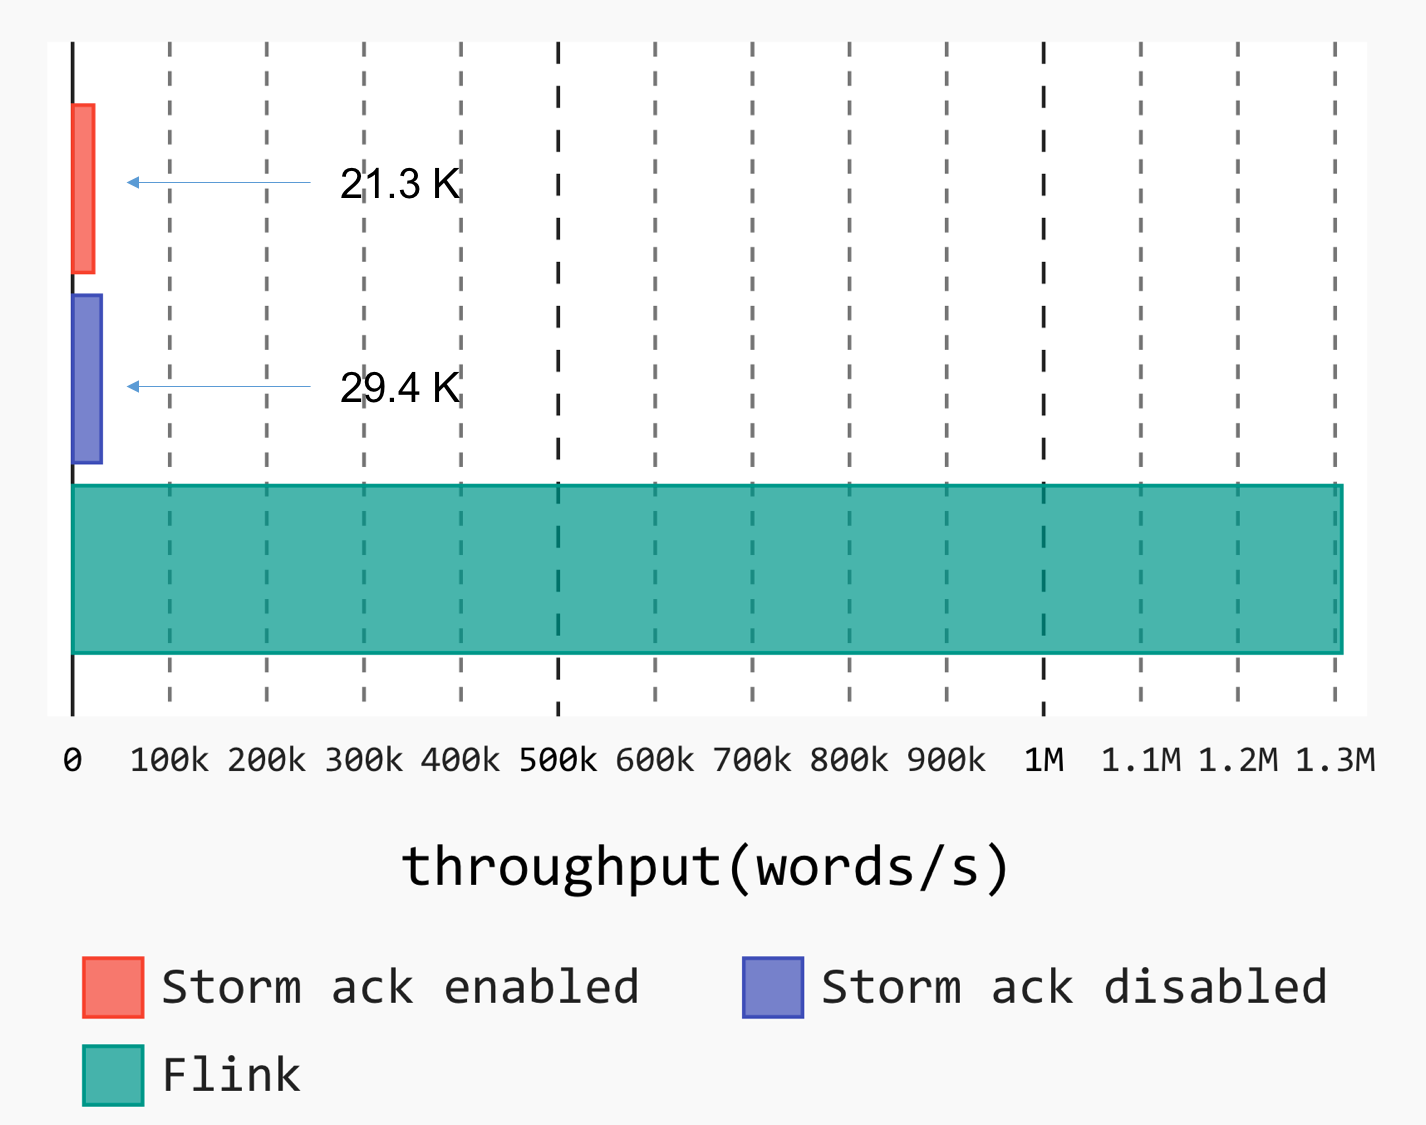
\includegraphics[scale=0.2]{images/throughput_skewed}}
  ~
  \subfigure{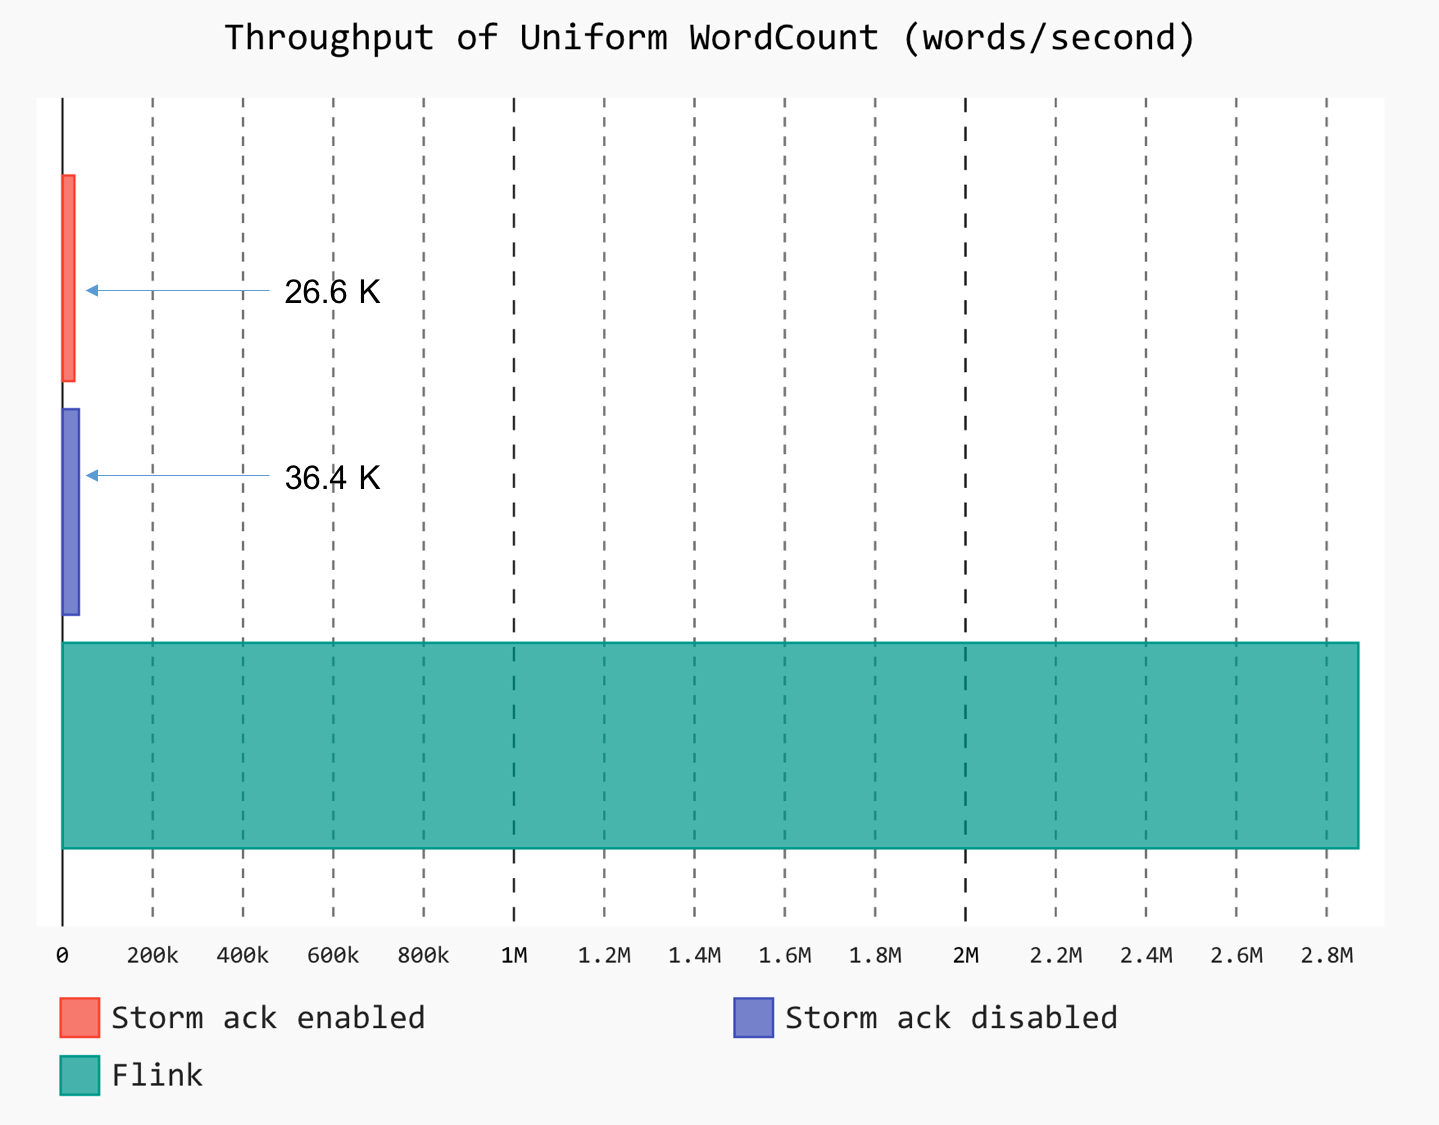
\includegraphics[scale=0.2]{images/throughput_uniform}}
   \caption{Throughput of Offline WordCount}
   \label{fig:offline_throughput}
  \end{center}
\end{figure}

Since the computing model of Spark Streaming is micro-batch processing. Existing data in Kafka cluster would be collected and processed as one single batch. The performance of processing one large batch with Spark Streaming is similar to a Spark batch job. There are already many works evaluating performance of Spark batch processing. Therefore, we skip experiments of Spark Streaming here. Figure~\ref{fig:offline_throughput} shows throughput of Storm and Flink clusters executing Offline WordCount with both skewed data and uniform data. It is obvious that the performance of Flink is much better than Storm, achieving around 50 to 100 times larger throughput. The throughput of Flink cluster processing uniform data stream up to 2.83 million words per second.  The skewness of experiment data has great influence of performance. The throughput of Flink cluster performing uniform data is more than two times as large as throughput of performing skewed data. The corresponding ratio of Storm is around 1.25. 

\begin{figure}[t!]
  \begin{center}
  \subfigure{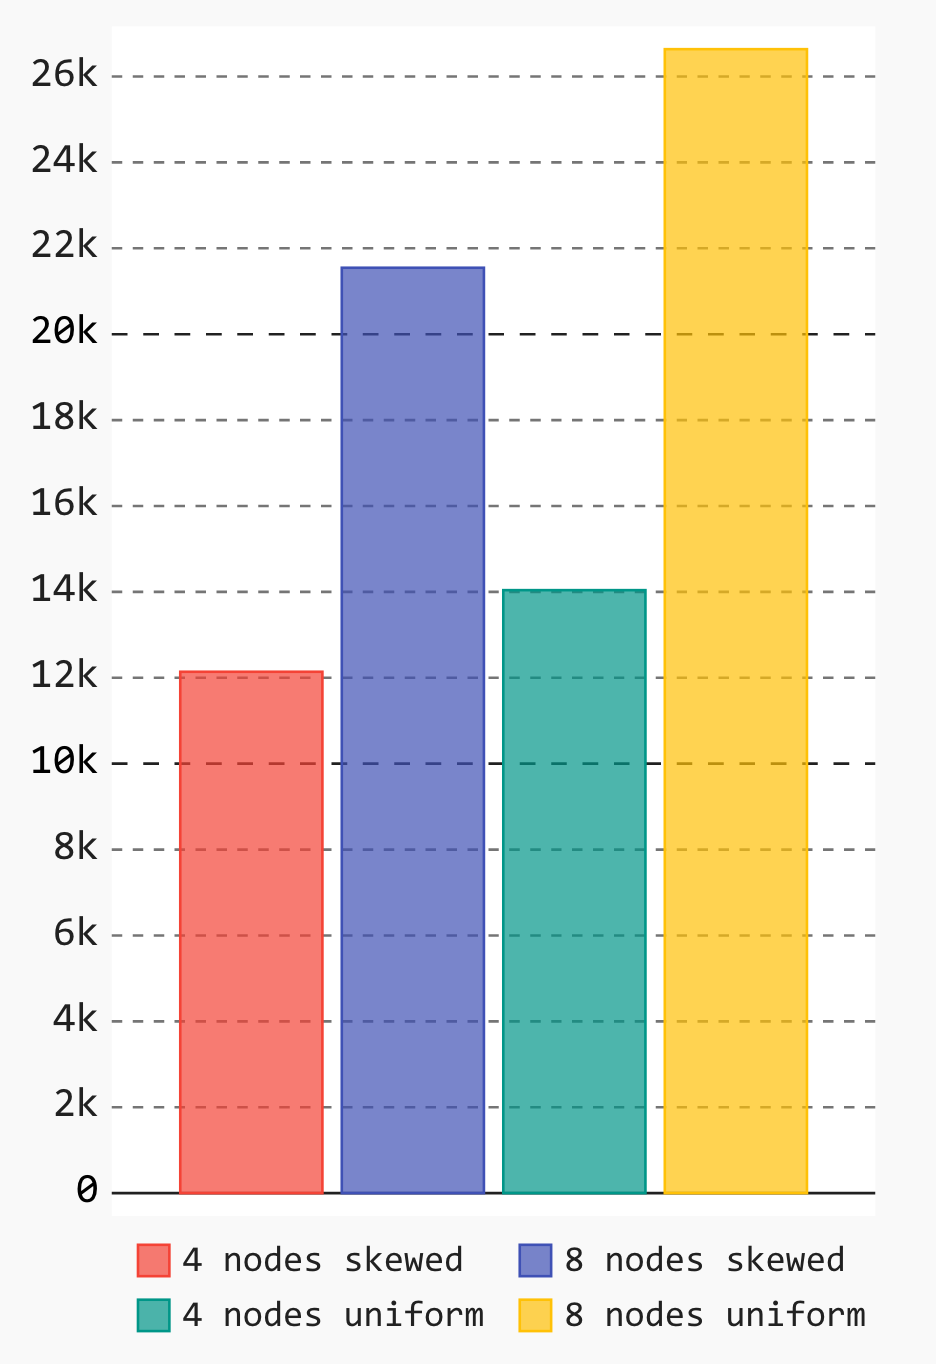
\includegraphics[scale=0.25]{images/storm_throughput_scale}}
  ~
  \subfigure{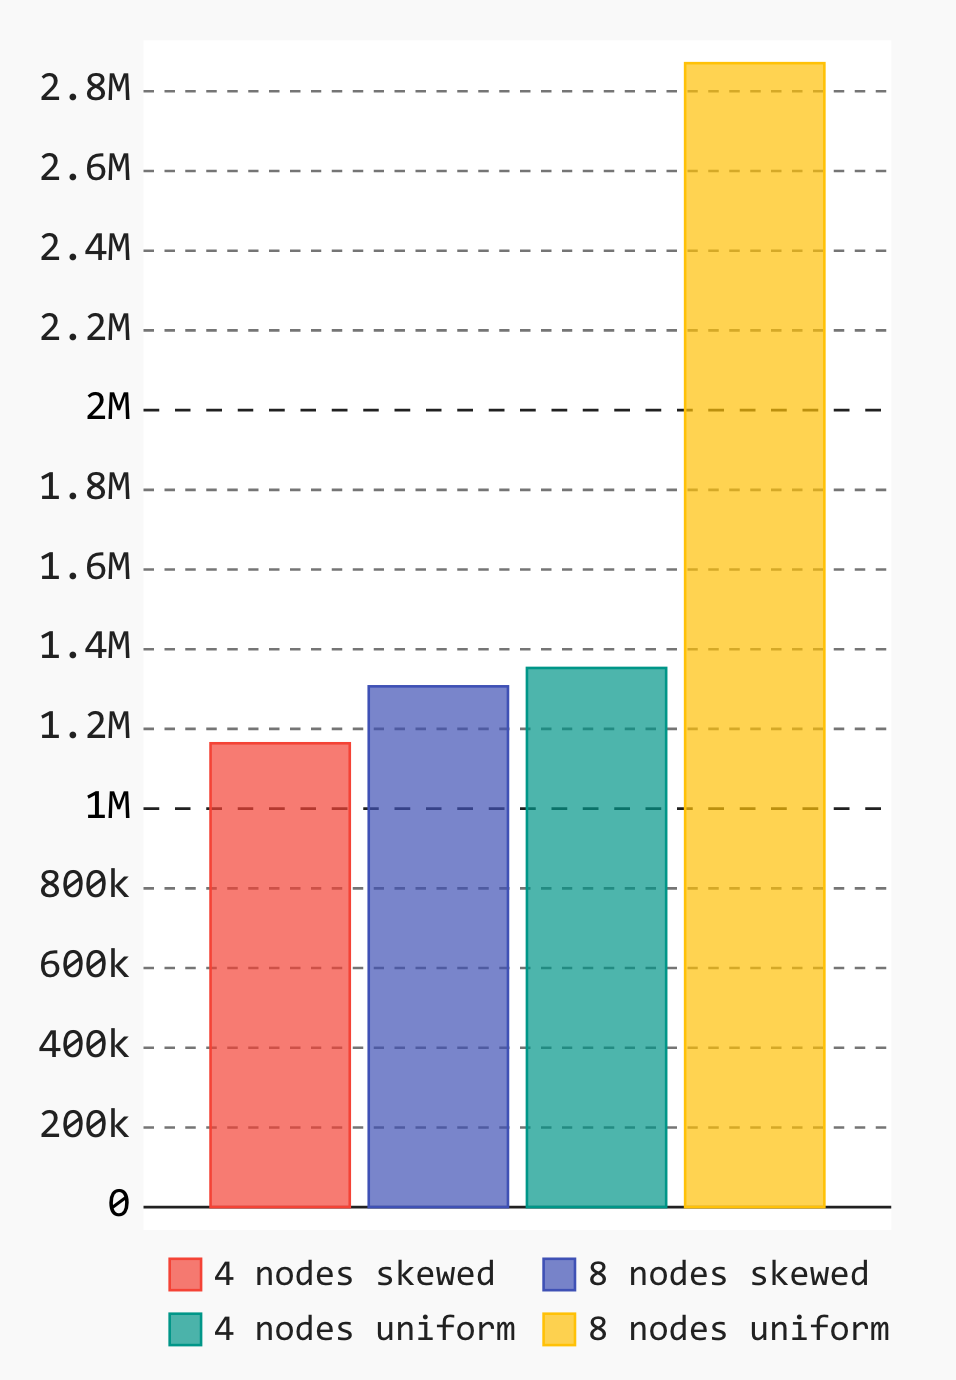
\includegraphics[scale=0.25]{images/flink_throughput_scale}}
   \caption{Throughput Scale Comparison of Offline WordCount}
   \label{fig:offline_throughput_scale}
  \end{center}
\end{figure}

The difference of performance between skewed data and uniform data indicates that the bottleneck of a cluster processing skewed data would be the node dealing with data with highest probability. To verify this assumption, we reduce the number of computing nodes from 8 to 4, and run these experiments. The experiment results are presented as Figure~\ref{fig:offline_throughput_scale}. The throughput of 8-nodes cluster of both systems dealing with uniform data is nearly two times as large as that of 4-nodes cluster. It means that the scalability of both systems is good. While processing skewed data, increasing the number of work nodes in a Flink cluster doesn't bring significant performance increase. Storm cluster gets about 58\% throughput improvement while increasing cluster from 4 nodes to 8 nodes. These results show that the assumption is correct with Flink and the bottleneck of a storm cluster might be other factors.

The throughput of each work node in computing cluster is displayed in Figure~\ref{fig:worknodes_throughput}. Obviously storm has lower throughput, but achieves better workload balance than Flink. The experiment results also shows that clusters with 4 compute nodes of both systems have better workload balance than clusters with 8 nodes and workloads preforming uniform data achieve better balance that corresponding workloads performing skewed data.


\begin{figure}[t!]
  \begin{center}
   \subfigure{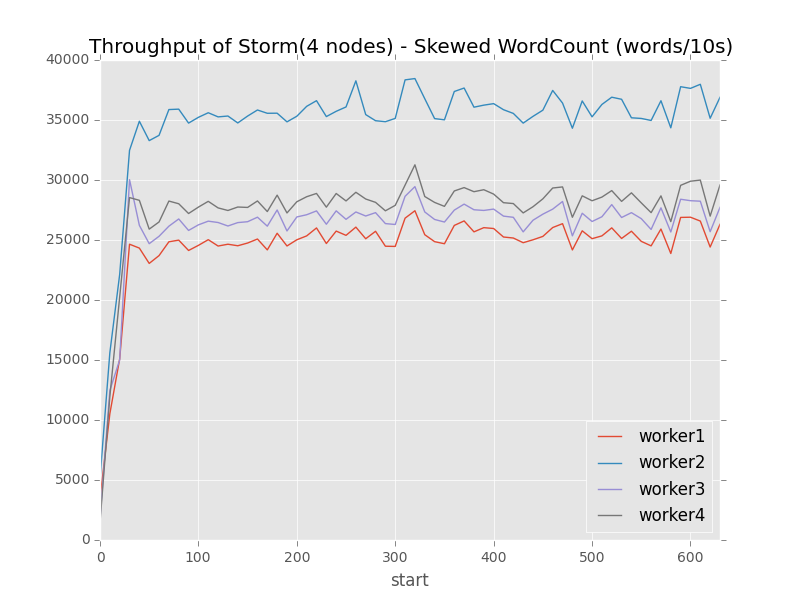
\includegraphics[scale=0.25]{images/storm4nodes_skewed_throughput}}
  ~
  \subfigure{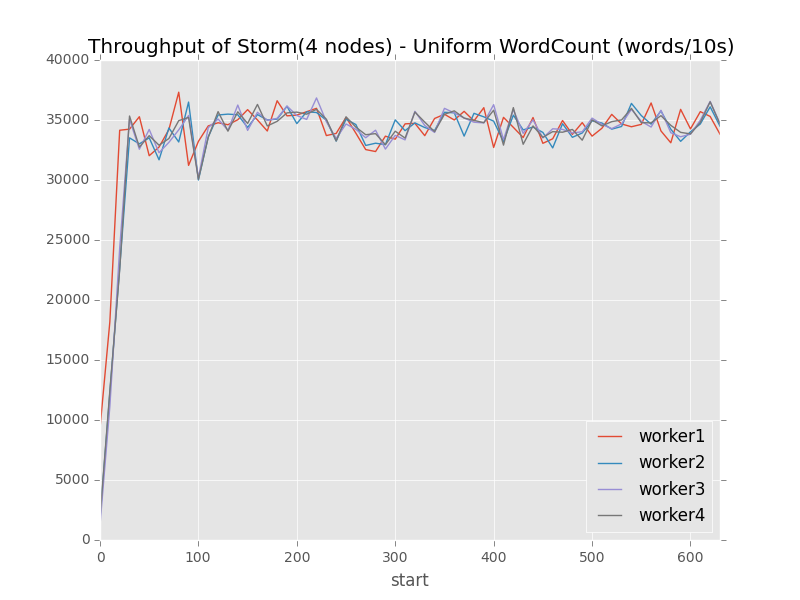
\includegraphics[scale=0.25]{images/storm4nodes_uniform_throughput}}
  ~
  \subfigure{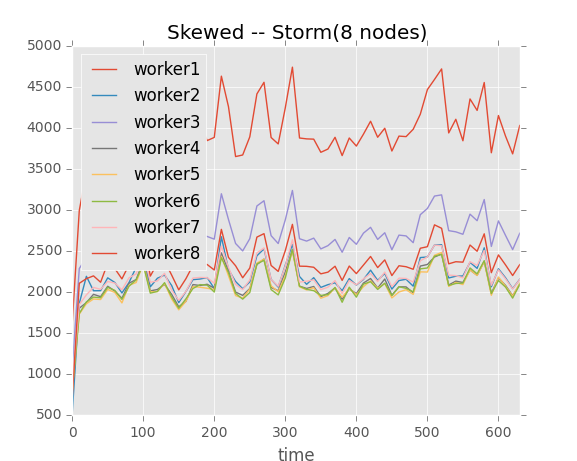
\includegraphics[scale=0.25]{images/storm_skewed_throughput2}}
  ~
  \subfigure{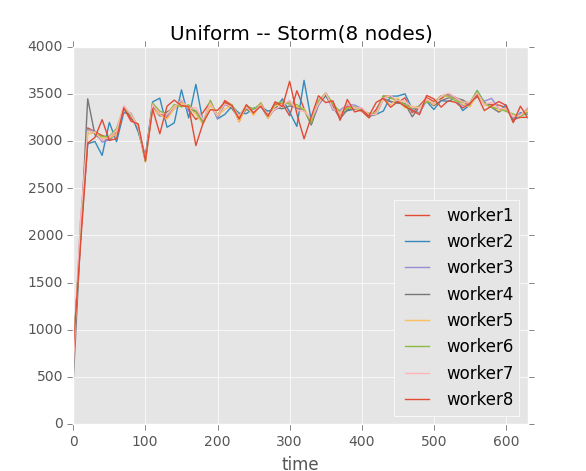
\includegraphics[scale=0.25]{images/storm_uniform_throughput2}}
  ~
    \subfigure{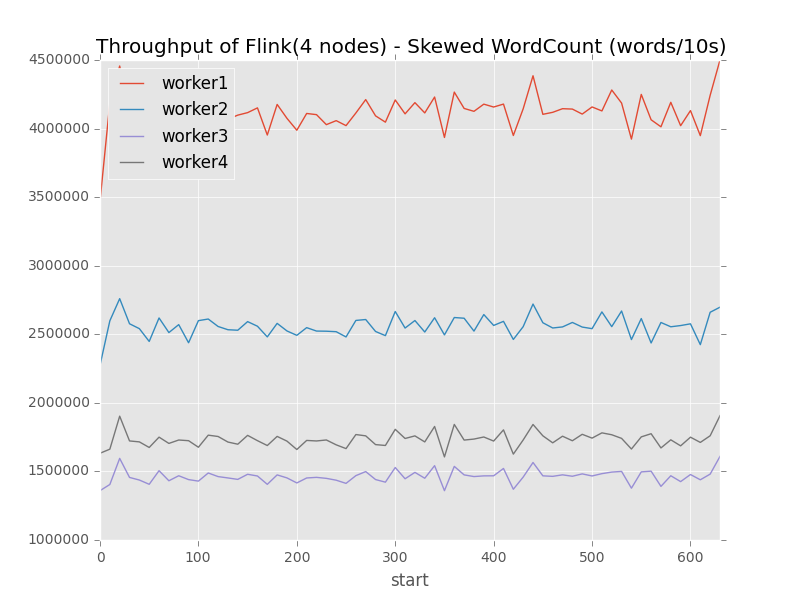
\includegraphics[scale=0.25]{images/flink4nodes_skewed_throughput}}
  ~
  \subfigure{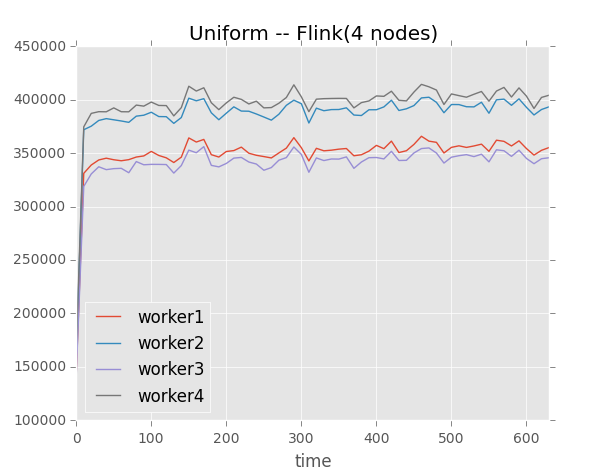
\includegraphics[scale=0.25]{images/flink4nodes_uniform_throughput}}
  ~
  \subfigure{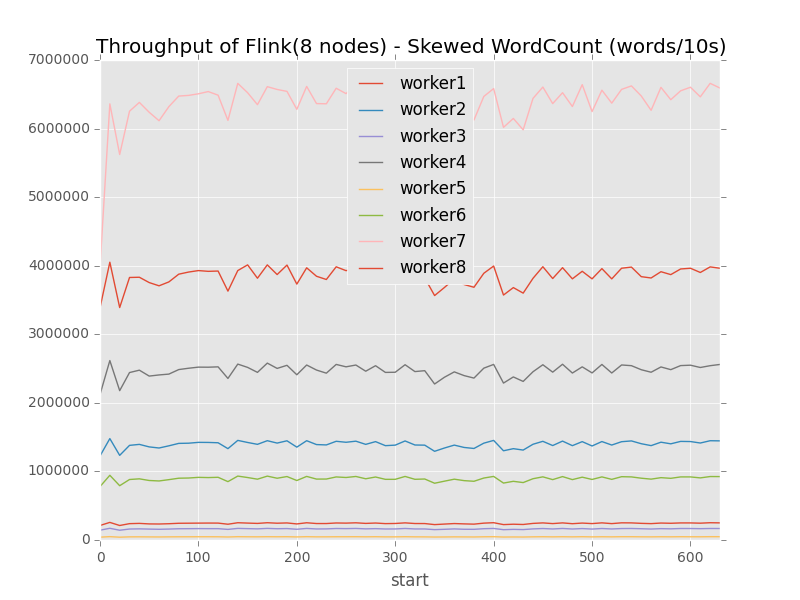
\includegraphics[scale=0.25]{images/flink_skewed_throughput}}
  ~
  \subfigure{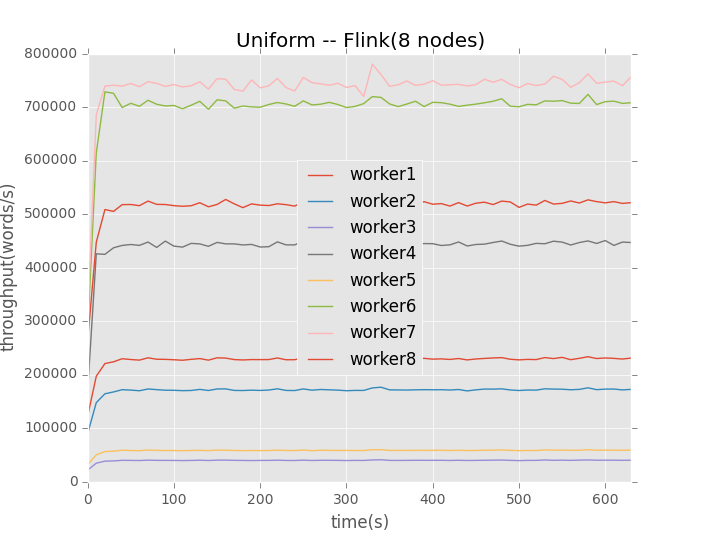
\includegraphics[scale=0.25]{images/flink_uniform_throughput}}

   \caption{Throughput of work nodes}
   \label{fig:worknodes_throughput}
  \end{center}
\end{figure}

\subsection{Online WordCount}
\label{subsec:online_wordcount}

Base on the experiment results of Offline WordCount, we perform experiments of Online WordCount on Storm and Flink at half throughput of Offline WordCount respectively.  As mentioned in \cref{section:log_statistic}, the latency is computed as spending time from a record generated to corresponding result computed. Storm with ack enabled achieves a median latency of 10 milliseconds, and a 95-th percentile latency of 201 milliseconds, meaning that 95\% of all latencies were below 201 milliseconds. Flink has a little higher median latency (53 milliseconds), and a 99-th percentile latency of 521 milliseconds that is close to Storm. 

\begin{figure}
  \begin{center}
  \subfigure{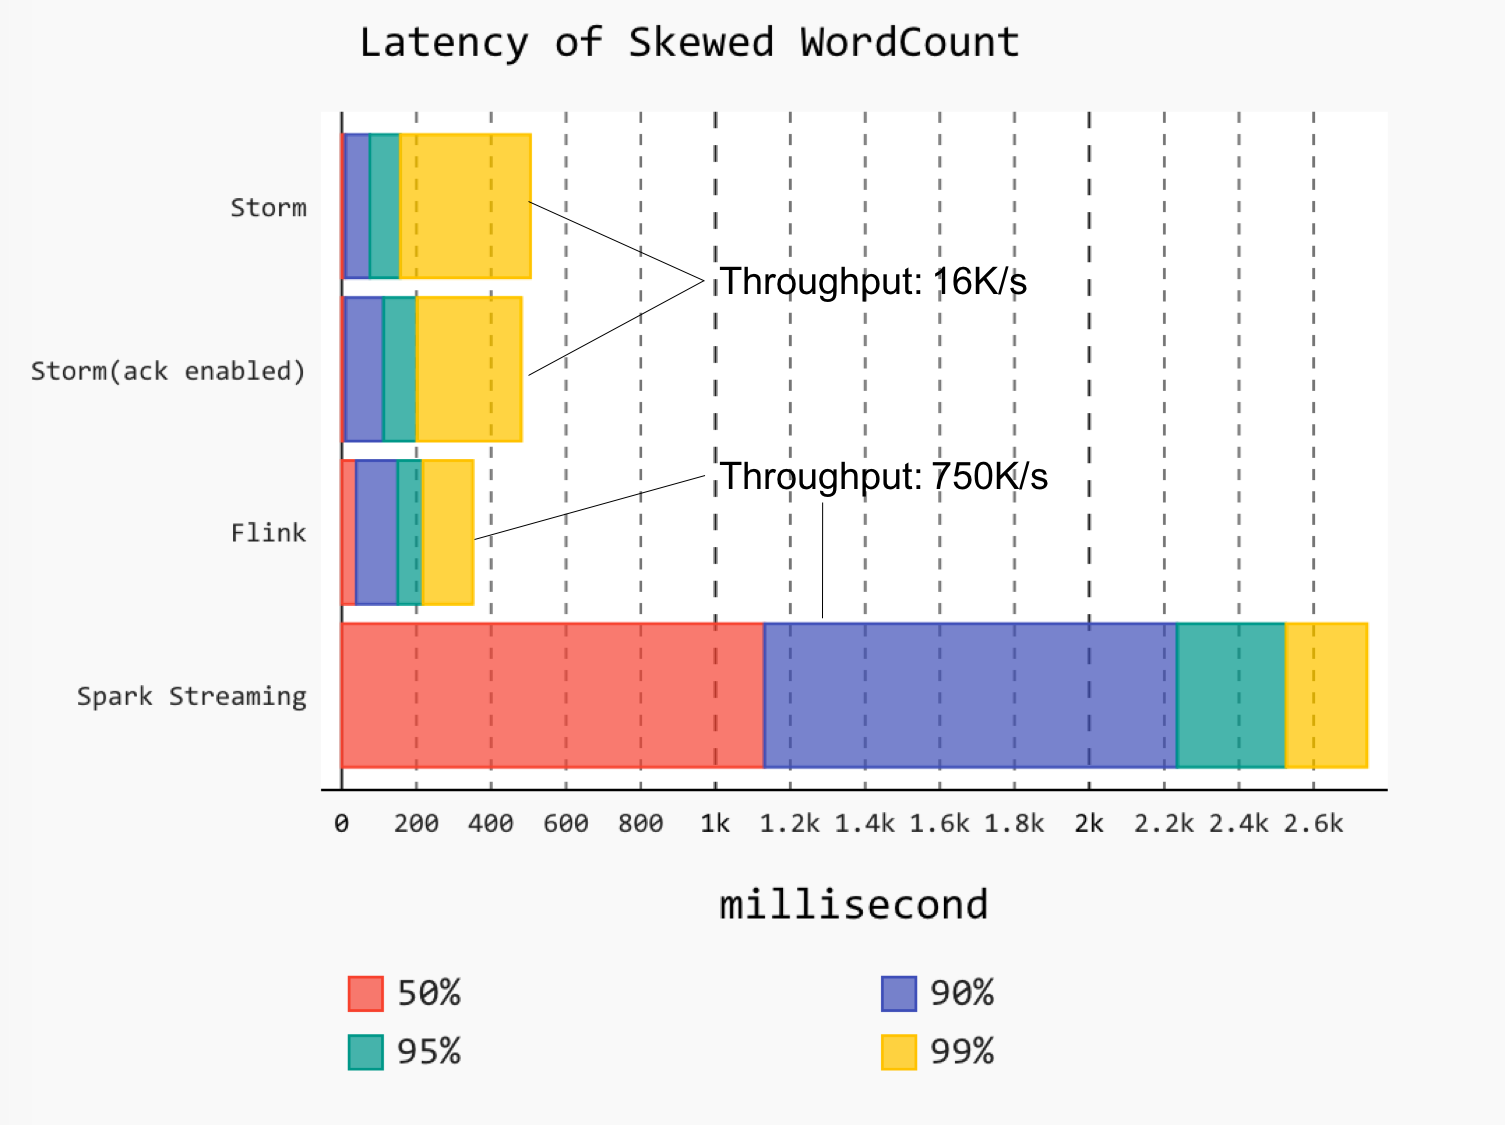
\includegraphics[scale=0.4]{images/latency_skewedwordcount}}
   \caption{Latency of Online WordCount}
   \label{fig:online_wordcount_latency}
  \end{center}
\end{figure}

In Spark Streaming, depending on the nature of the streaming computation, the batch interval used may have significant impact on the data rates that can be sustained by the application on a fixed set of cluster resources\footnote{\url{http://spark.apache.org/docs/1.5.1/streaming-programming-guide.html\#setting-the-right-batch-interval}}. Here, we perform the experiments with one second micro-batch interval and 10 seconds checkpoint interval which are the default configurations. Checkpointing is enabled because of a stateful transformation, \texttt{updateStateByKey} is used here to accumulate word counts.  Checkpointing is very time consuming due to writing information to a fault- tolerant storage system. Figure~\ref{fig:spark_wordcount_latency} shows that the latency of micro-batches processing increasing and decreasing periodically because of checkpointing. The throughput of experiment corresponding to Figure~\ref{fig:spark_wordcount_latency} is 1.4M/s (million words per second) of skewed data. When the speed of data generation reaches 1.8M/s, the delay and latency increase infinitely with periodic decreasing.

As mentioned in \cref{sub:basic_operator}, we designed another version of WordCount named Windowed Wordcount. Actually, Spark Streaming supports pre-aggregation by default, therefore, above Spark Streaming WordCount experiments already own this feature. Currently, Flink-0.10.1 doesn't support pre-aggregation and parallel window could only be applied on keyed stream. It is possible to implement Windowed WordCount with Flink's low level API. But it is too time consuming and we leave it to future works. Therefore, only Storm is benchmarked with this workload.

\begin{figure}
  \begin{center}
  \subfigure{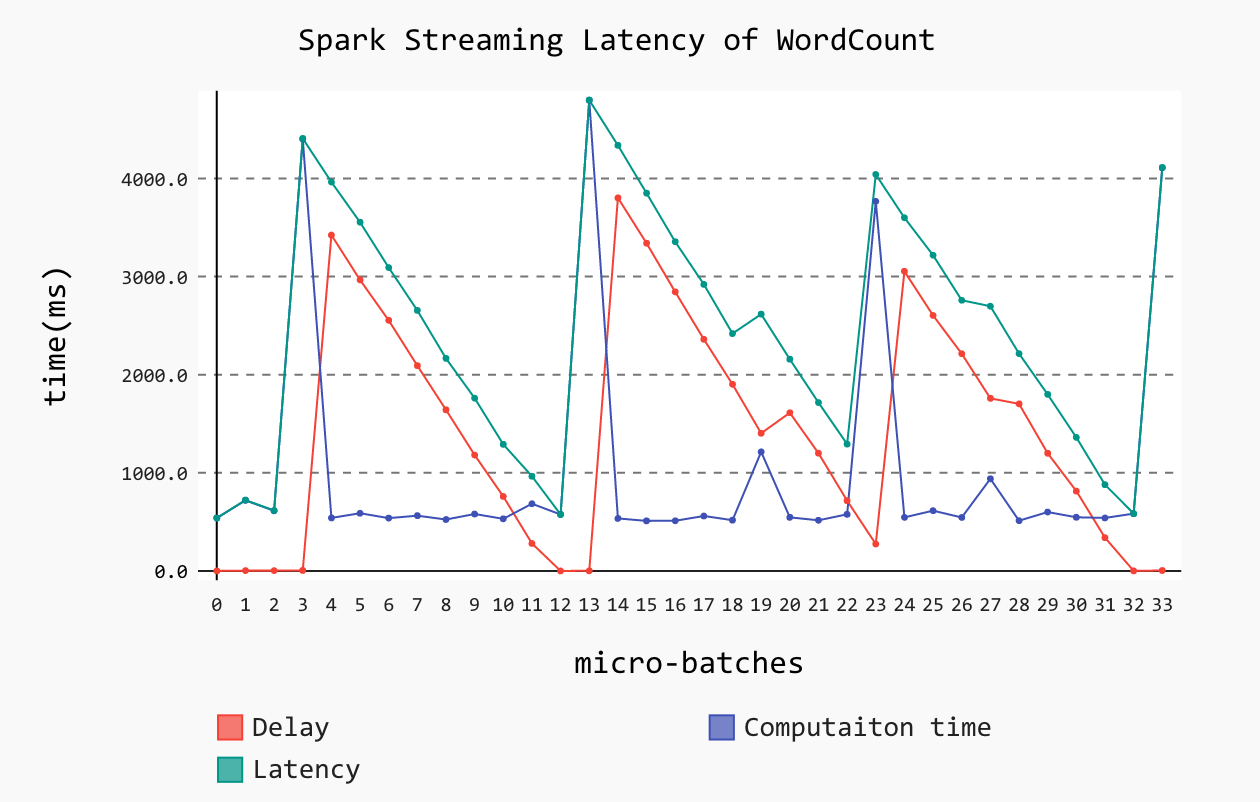
\includegraphics[scale=0.2]{images/spark_wordcount_latency}}
   \caption{Spark Streaming WordCount Latency}
   \label{fig:spark_wordcount_latency}
  \end{center}
\end{figure}

To support Windowed WordCount, we implemented a \texttt{window} operator in Storm\footnote{\url{https://github.com/wangyangjun/Storm-window}}. From our experiments, the window time has very limit effect on throughput. Here only experiment results of one second window workload are presented. The throughput of Windowed WordCount performing skewed data in Offline model could reach 60K/s (thousand words per second) that is more than two times as large as experiments without window. While dealing with uniform data, the throughput doesn't have any obvious improvement. Online model with a generation speed of 50K/s achieves a median latency of 1431 milliseconds, and a 99-th percentile latency of 3877 milliseconds.


\section{AdvClick}

\begin{figure}
  \begin{center}
  \subfigure{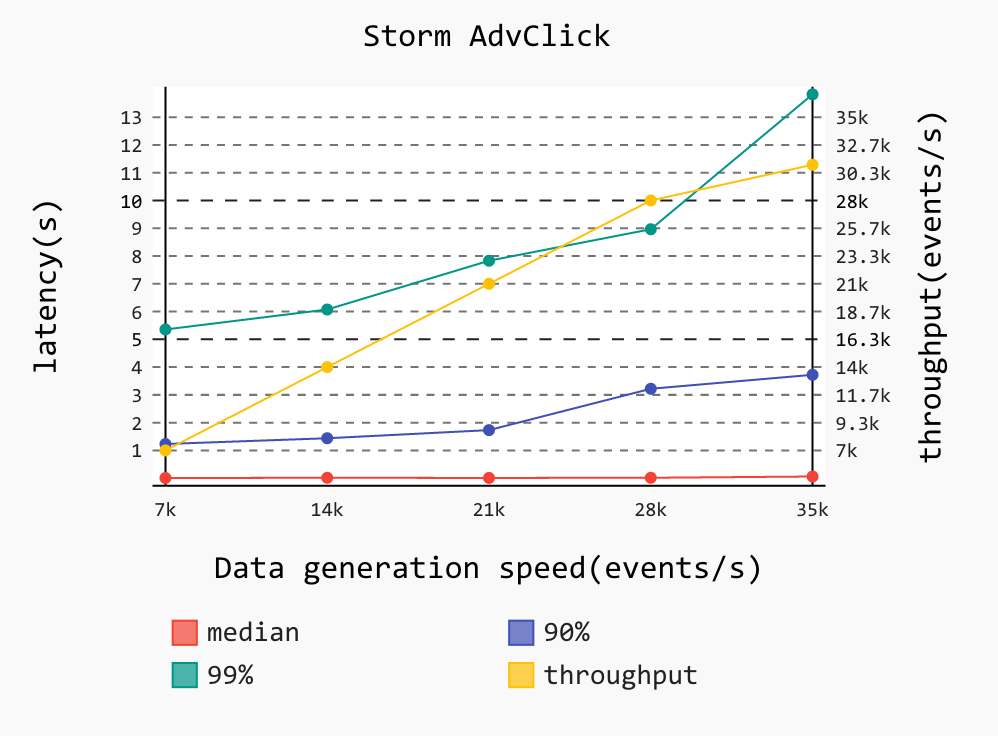
\includegraphics[scale=0.2]{images/storm_adv_latency}}
   \caption{Storm AdvClick Latency}
   \label{fig:storm_adv_click}
  \end{center}
\end{figure}

As described in \cref{subsection:advclick_generator}, click delays of clicked advertisements satisfy normal distribution and the mean is set to 10 seconds. In our experiments, we define that clicks in 20s after corresponding advertisement shown are valid clicks. In theory, overwhelming majority records in stream \texttt{click} could be joined. Kafka only provides a total order over messages within a partition, not between different partitions in a topic\cite{Kafka}. Therefore, it is possible that click record arrives earlier than corresponding advertisement shown record. We set a window time of 5 seconds for \texttt{advertisement clicks} stream.

When benchmarking Storm and Flink, first we perform experiments with low speed data generation and then increase the speed until obvious joining failures occur when throughput is much less than generation speed of stream \texttt{advertisement clicks}. The experiment result shows that the maximum throughput of Storm cluster is around 8.4K/s (joined events per second). The corresponding generation speed of \texttt{shown advertisements} is 28K/s. Figure~\ref{fig:storm_adv_click} shows that Storm cluster has a very low median latency. The 90-th percentiles of latency are all between one second and two seconds. But the 99-th percentile of latency are much higher and increase dramatically with the data generation speed.

\begin{figure}
  \begin{center}
  \subfigure{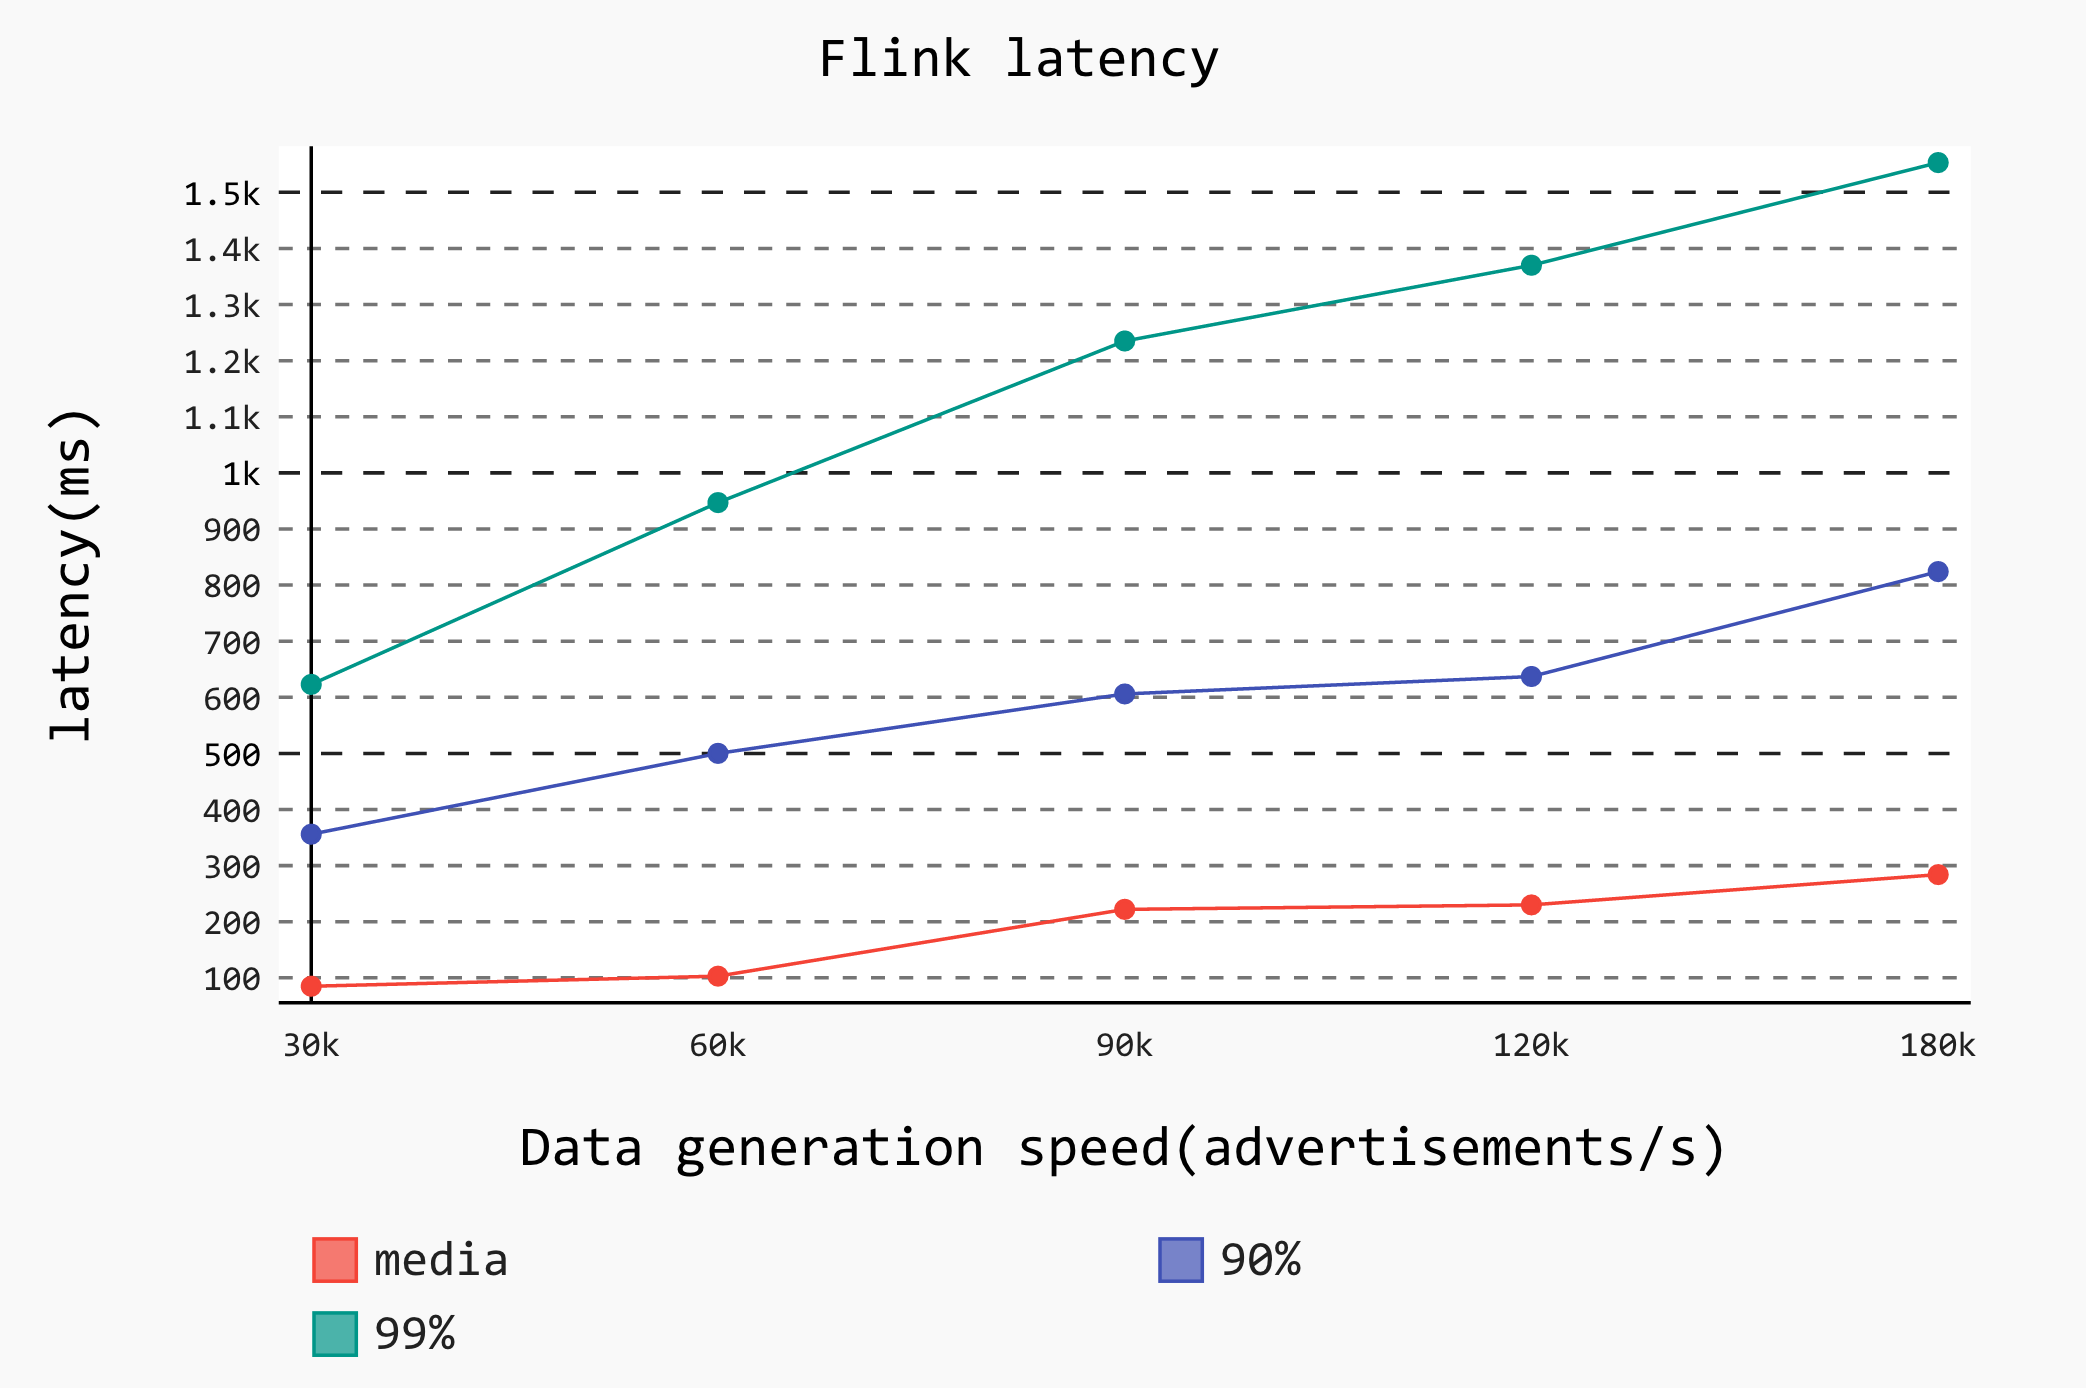
\includegraphics[scale=0.2]{images/flink_adv_latency}}
   \caption{Flink AdvClick Latency}
   \label{fig:flink_adv_click}
  \end{center}
\end{figure}


Compare to Storm, Flink achieves much better throughput. When generation speed of stream \texttt{shown advertisements} increases from 180K/s to 210K/s, Flink cluster stops consuming data from Kafka. The maximum throughput of Flink is between 54 K/s and 63K/s, around 6 times larger than Storm. The latency of Flink performing this workload is shown as Figure~\ref{fig:flink_adv_click}. Even though the median latencies are a little higher than Storm, but 90-th and 99-th percentiles of Flink latency are much lower. 

In this workload, window length of stream \texttt{show advertisements} and \texttt{advertisement clicks} are 20 seconds and 5 seconds respectively. As discussed in \cref{sub:join_operator}, Spark Streaming join operator is applied with sliding window. With the configuration of 20s/5s, the slide intervals of both windows are 5 seconds. That means a micro-batch join job is submitted to Spark Streaming cluster every 5 seconds. Because of different processing model, there is no joining failure in Spark Streaming. But high data generation speed leads to increasing delay of micro-batch jobs because the previous micro-batch jobs couldn't be finished in interval time. With this configuration, Spark Streaming has a very small throughput which is lower than 2K/s. Increasing micro-batch jobs submitting interval might increase the throughput, but leads to higher latency. For this workload, increasing the window lengths also gives ups correct results. Therefore, we did some experiments with larger windows. Increasing windows length of these two streams to 60s/30s, the cluster could achieve a throughput of 20K/s.


\section{K-Means}

Experiment results of stream k-means processing 2-dimensional points shows that Storm cluster with at-least-once processing guarantee has a throughput of 1.7K/s and median latency of 500ms. Without this guarantee, the throughput is similar, but achieves better median latency of 10ms. The throughput of Flink cluster is about 78K/s. Figure~\ref{fig:kmeans_latency} shows the latencies of Storm and Flink clusters operating at half size of corresponding max throughput. Both Storm with and without at-least-once guarantee achieve very low median latency and a much higher 99-th percentile latency. Generally, the latency of Storm with at-lest-once guarantee is a little higher. Compare with Storm, latency percentiles of Flink is more compact. Flink achieves a median latency of 122 milliseconds, and a 99-th percentile latency of 310 milliseconds, meaning that 99\% of all latencies were below 310 milliseconds. 
 
\begin{figure}
  \begin{center}
  \subfigure{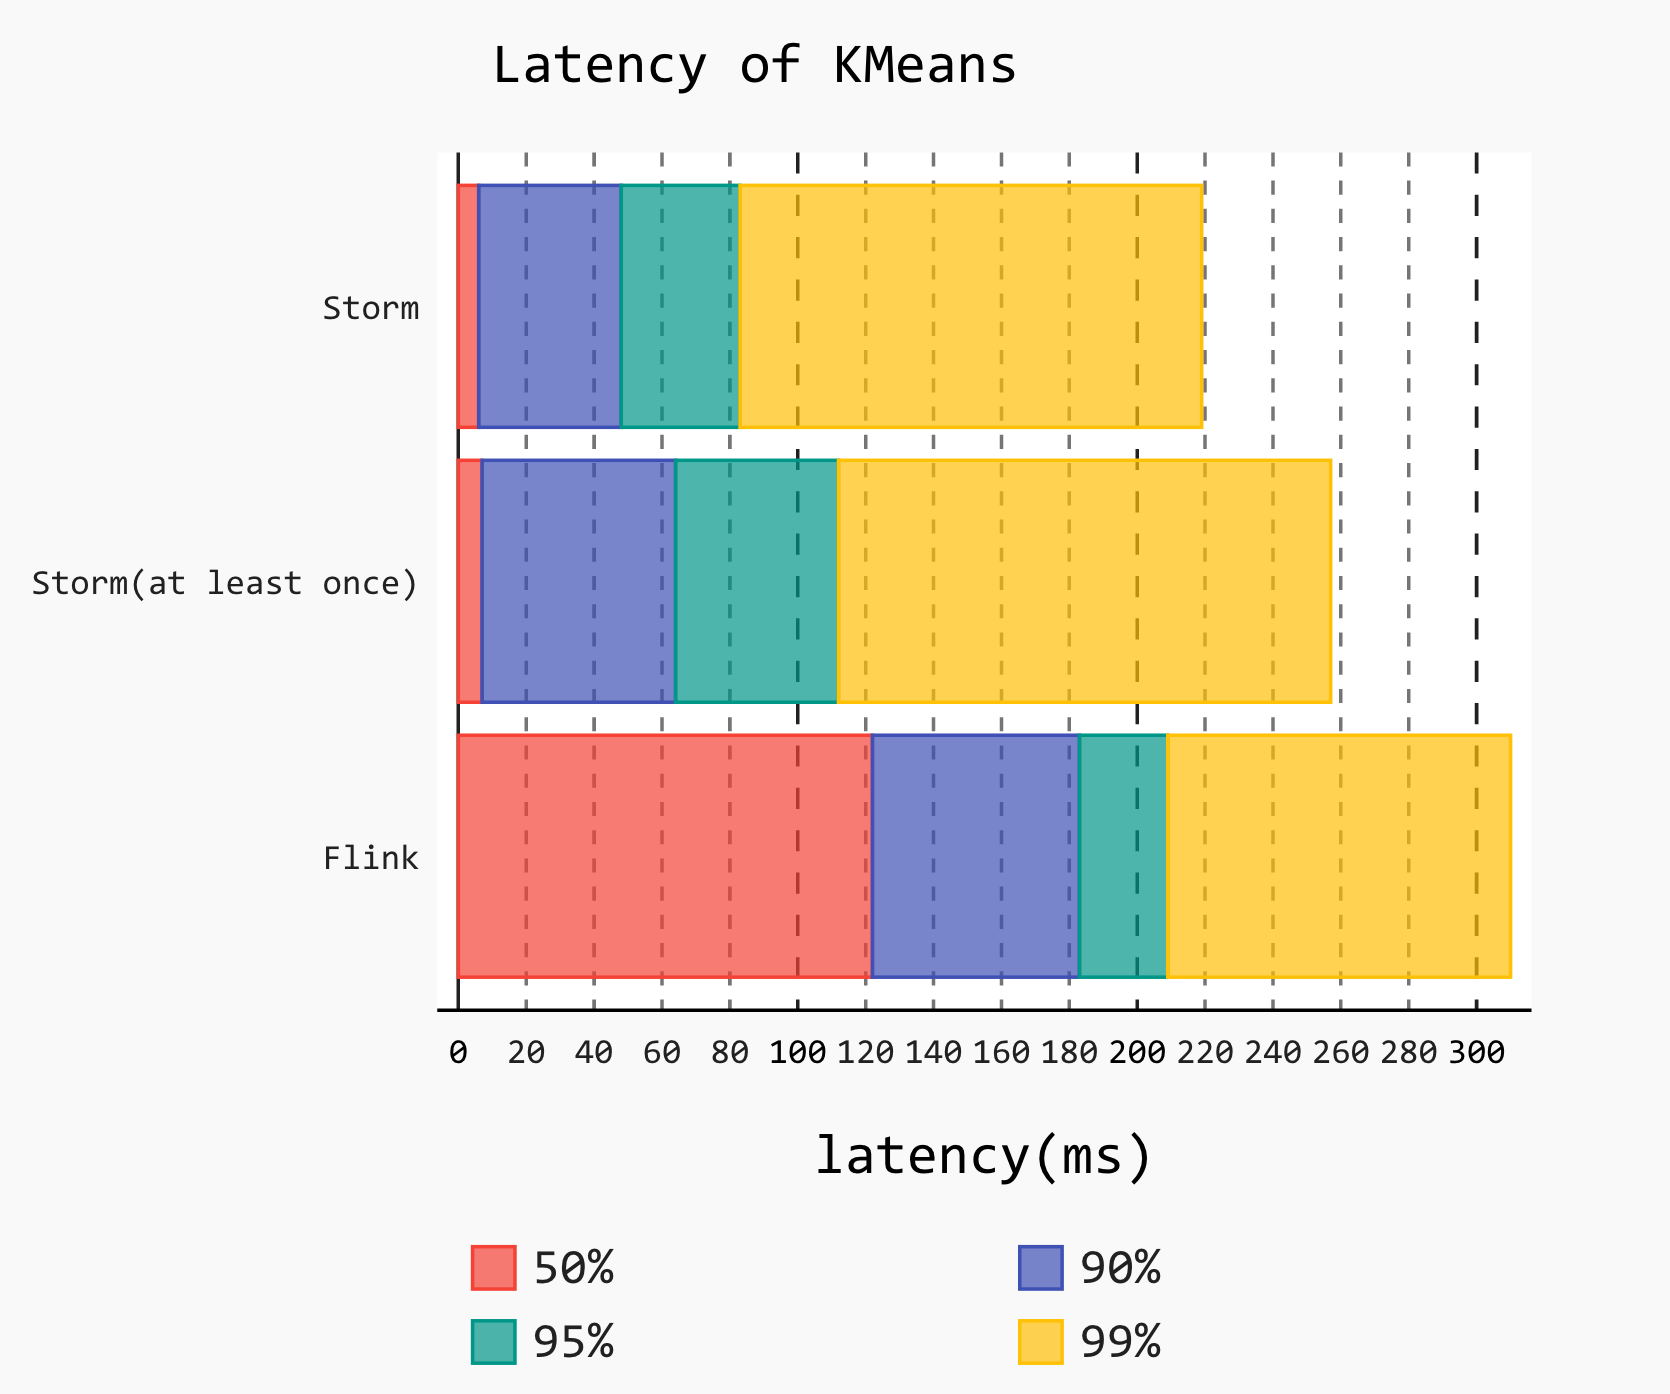
\includegraphics[scale=0.25]{images/kmeans_latency}}
   \caption{KMeans Latency}
   \label{fig:kmeans_latency}
  \end{center}
\end{figure}

% convance
Since the throughput of Flink is tens of times higher than Storm, this workload converges much quicker on Flink cluster. In order to compare convergences of the algorithm running on Storm and Flink clusters, we calculated average distance between centroids and corresponding nearest center base on the number of points processed on each compute node and visualized as Figure~\ref{fig:converge}. The results indicate that the k-means algorithm performing on Storm cluster achieves better convergence.

\begin{figure}
  \begin{center}
  \subfigure{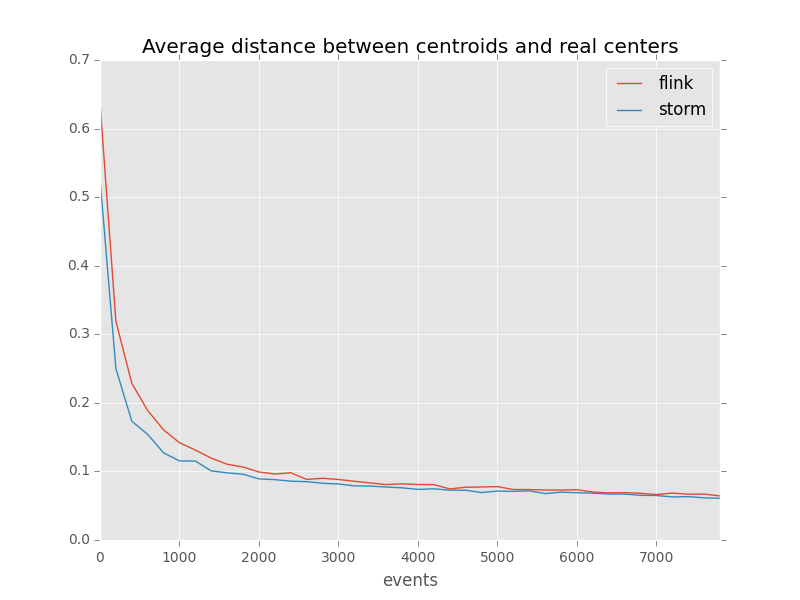
\includegraphics[scale=0.35]{images/converge}}
   \caption{Convergence base on processed points }
   \label{fig:converge}
  \end{center}
\end{figure}

% dimension
Our experiment results show that increasing point dimension had very limit effect on workload performance, which indicates that computation is a bottleneck of this workload.

\clearpage

